\documentclass{article}
\usepackage{amsmath}
\usepackage{graphicx}
\graphicspath{{./images/}}

\begin{document}
\author{Hawley, Adam}
\title{Lecture 3: Photometric Image Formation\\Part 2}

\maketitle
\tableofcontents
\newpage

\section{Brightness}
Light reaches the camera from a scene. 
The amount of light arriving from the scene depends on what is in the scene (strength of light sources, reflectance properties of objects in the scene etc). 
The pixel brightness reported in an image for a given scene radiance quantity depends on the {\it exposure} of the image. 
A camera can control {\it exposure} in a number of ways.

\subsection{Formulae}
Before discussing the several parameters which can be adjusted to increase total exposure, there are a couple of formulae to be explained and understood first.

\begin{itemize}
	\item {The amount of light captured by a lens is proportional to the area of the aperture:

\centerline{$Area = \pi(\frac{D}{2})^2$}

D is the diameter of the entrance pupil.}

\item {The {\bf f-number}(N) is the ratio of the focal length (f) to the diameter of the entrance pupil:

\centerline{$N = \frac{f}{D}$}

The higher the f-number, the less light that reaches the CCD (smaller diameter)}

\end{itemize}

Substituting D gets:

\centerline{$Area = \pi (\frac{f}{2N})^2$}

\begin{itemize}
	\item Area is proportional to the reciprocal square of the f-number
	\item Photographers have found it convenient to define a discrete set of f-numbers as ``stops''.
	\item Each stop represents a halving of area of the aperture relative to the previous stop.
\end{itemize}
\begin{align*}
	A_1 &= 2\cdot A_2 \\
	\frac{\pi(d_1)^2}{4} &= 2\cdot \frac{\pi(d_2)^2}{4} \\
	(d_1)^2 &= 2\cdot (d_2)^2 \\
d_2 = \sqrt{(d1)^2\cdot\frac{1}{2}} &= (d_1)\cdot \frac{\sqrt{1}}{\sqrt{2}} = \frac{d_1}{\sqrt{2}}
\end{align*}
Therefore to halve the area of the aperture the f-number must be multiplied by \\ 
\centerline{$\sqrt{2} \approx 1.4$.} \\
Hence, the set of stops is:\\
\centerline{$\frac{f}{1}, \frac{f}{1.4}, \frac{f}{2}, \frac{f}{2.8} ...$}

Each stop represents a halving of the light intensity from the previous stop. 
Hence aperture gives us one way to control how much light reaches the camera.
However, as one changes the aperture, other complex effects are introduced.

As the f-number reduces (aperture gets larger, more light enters lens), ``depth of field'' gets smaller and sharp focus is only possible for a limited range of distances. 


\subsection{Aperture}
{\it Aperture} is the first parameter which can change the overall light exposure onto the CCD. 
The {\it aperture} of a camera is the hole through which light travels. 
Aperture size determines the cone angle of a bundle of rays that come to focus in the image plane. 

\begin{itemize}
	\item Small aperture = less light and more highly collimated rays admitted, sharp focus at image plane.

	\item Large aperture = more light and uncollimated rays admitted, sharp focus only for rays with a certain focal length.
\end{itemize}

Aperture sizes are measured in units of {\it stops} with cameras offering a discrete set of aperture sizes.

\subsection{Exposure}
Exposure is the accumulated physical quality of light applied to the image-plane over a given time.

Product of the image irradiance (light arriving at the CCD) and time: 
\centerline{$H = E\cdot t$}

{\bf Note:} In practice, cameras apply a non-linear transformation to intensities so the discretised pixel values will be a function of H. However, this is ignored under the {\it ``linear camera''} assumption.

Hence, another way to control how much light reaches the CCD is to change the exposure time.

However, increasing the exposure can cause motion blur and dark current noise (see Lecture 3 notes) will also increase with time.

\subsection{Gain}
The brightness of an image can also be increased by passing the analogue signal from the CCD through an amplifier.
The signal gain of a camera is measured on the {\it ``ISO''} scale.
Increasing ISO from its default value of 100 corresponds to increasing signal gain.
Modern CCDs can support incredibly high ISO values and hence operation in very low light.
Remember, increasing the gain will not affect any saturated pixels, they will simply remain saturated.

\subsection{Summary}
To summarise, there are three main ways one can increase the brightness of an image:

\begin{itemize}
	\item Increasing the aperture (smaller f-number). (Reduced depth of field)
	\item Longer exposure (motion blur is worsened).
	\item Increasing the gain through a large ISO (noise is also amplified)
\end{itemize}
\section{High Dynamic Range Imaging}
\subsection{History}
\begin{itemize}
	\item {\bf 1850s}: Gustave Le Gray - Chemical process for combining two exposures.
	\item {\bf 1950s}: ``Dodging and burning'', during film development, make local adjustments to sensitivity.
	\item {\bf 1988-1993}: Technion, Israel --- local tonemapping, first HDR video.
	\item {\bf Modern HDR}: Global HDR {\bf (1993)} --- idea of combining images to compute a global luminance map then tonemap, Debevac et al. {\bf (1997)} --- the method explained below. 
\end{itemize}

\subsection{HDR --- How is it done today?}
High dynamic range imaging captures a sequence of images with different exposures. 
Combining the images captures a much wider dynamic range.
The brightness of pixel $i$ in image $j$ is given by:
\begin{align*}
	H_{ij} &= E_i \cdot t_j \\
	\log(H_{ij}) &= \log(E_i) + \log(t_j)
\end{align*}
\begin{itemize}
	\item $t$ is varied for each image
	\item $H$ are the known pixel values
	\item $E$ are the unknown pixel radiances
\end{itemize}

Each image gives us an estimate of the radiance at a pixel.
\begin{align*}
	\log(E_i) = \log(H_{ij}) - \log(t_j)
\end{align*}
The pixel brightness tells us something about how reliable the estimate is:
\begin{itemize}
	\item $\approx 255$ If a pixel is very bright (close to being saturated then the estimate is unreliable.
	\item $\approx 0$ If a pixel is very dark it will be noisy and unreliable. 
\end{itemize}
We give more weight to pixel values near the middle of the range:
\begin{figure}[!h]
	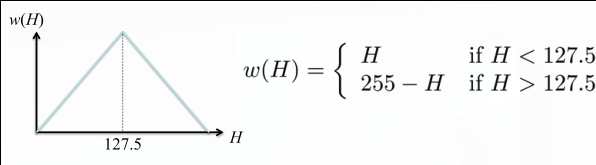
\includegraphics [width=\textwidth]{hdrweights.png}
	\caption{Formula for calculating weights based on pixel value}
	\label{Fig:hdrweights}
\end{figure}
To estimate the true radiance at every pixel we then simply take a weighted average of the estimates from each image:
\begin{align*}
	\log(E_i) &= \frac{\Sigma^K_{j=1}\omega(H_{ij})(\log(H_{ij})-\log(t_j))}
	{\Sigma^K_{j=1}\omega(H_{ij})}
\end{align*}
Saturated pixels are completely excluded. Radiance estimates for a pixel come from images where the exposure is appropriate for the scene radiance.
For colour images, separate channels can be processed independently.

\section{Tonemapping}
\subsection{Gamma Compression}
{\it Gamma compression} is an effective global (same function applied to all pixels) technique.
\begin{align*}
	I_{tonemapped} = cE^\gamma
\end{align*}
\begin{itemize}
	\item $c$ is a constant scaling where $c>0$.
	\item $\gamma$ is a constant that determines the contrast of the image where $0<\gamma<1$.
\end{itemize}
\subsection{Gradient-based Techniques}
The best techniques are local (output colour only depends on the local region around the pixel).
Gradient-based techniques try to preserve local gradient with less concern about overall brightness.
This means that they solve for a set of brightness values that minimises error in gradient while remaining between max and min allowable values.
\end{document}

